\documentclass[MasterThesisMain.tex]{subfiles}
\begin{document}
	\chapter{Experimental method}\label{experimentalmethod}
	
	\section{Polymers}
	
\section{The Experimental Setup}
The experimental setup is comprised of a NanoCalc XR and a Halogen light source(HL-2000-FHSA) which can produce wavelengths of \SI{360}{\nano\meter} to \SI{2400}{\nano\meter}. When the samples are being measured they are either placed on the ocean optics single point stage(ADD PICTURE) or in the test chamber(ADD PICTURE) made by the RUC workshop/machinists for x-ray scattering experiments. The NanoCalc is comprised of a spectrometer and an internal light source as seen in the figure \ref{fig:nanocalcsetup}, which can produce wavelengths of \SI{250}{\nano\meter} to \SI{1050}{\nano\meter} and measure thicknesses of \SI{10}{\nano\meter} to \SI{100}{\micro\meter}. The NanoCalc XR is connected to a computer where the NanoCalc software is installed and operated. For the experiments the halogen light source is used since it has a larger output power then the internal light source of the NanoCalc XR. The larger intensity output is need when performing experiments in the test chamber. To reiterate, white light is produced in the light source(HL-2000-FHSA), which travels through optical fiber and strikes that sample. The reflected light travels back through the optical fiber and the intensity across every wavelength of the white light is collected in the spectrometer and is sent to the NanoCalc software.  
	
	\begin{figure}
	\centering
		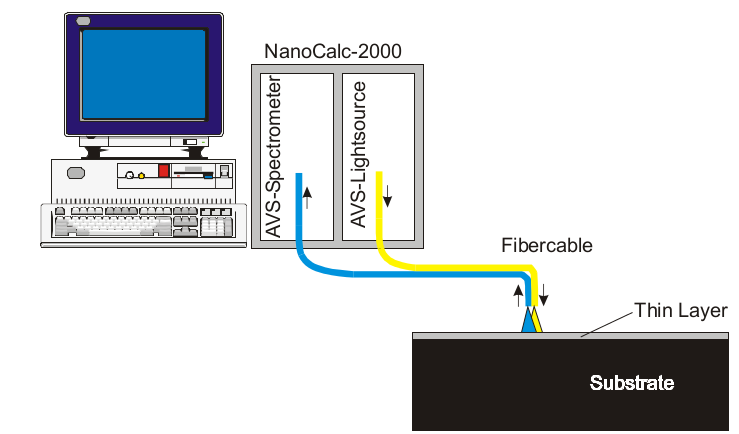
\includegraphics[width=\textwidth]{nanocalcsetup.png}
		\caption{This figure describes the NanoCalc set-up and has been taken from \cite{nanocalcmanual}. Light from a light source travels down the optical fiber illuminating the sample. The reflected light is collected by the optical fiber and analysed in the spectrometer. The spectrometer is connected to the computer by USB and the data is stored, modelled and manipulated through the NanoCalc software.}
		\label{fig:nanocalcsetup}
	\end{figure}
	
\section{Reflectance measurements in the NanoCalc spectrometer}
The NanoCalc spectrometer measures three light intensities which will be called a measurement onwards. The three measurements are the dark measurement (dark), the reference measurement (ref) and the thin-film measurement (meas). The dark measurement is the amount of light received by the optical fiber from external sources. The reference measurement is the amount of light reflected from a blank silicon wafer and the thin film measurement is the amount of light reflected from the sample. From chapter \ref{ch:reflect/trans}, the reflectance of a sample can be expressed as :

\begin{equation}\label{eq:nanocalcrefl}
R_{sample} = \frac{I_{sample}}{I_{incident}}
\end{equation}

The spectrometer does not measure the intensity of the incident light, therefore the reflectance of the substrate is used to isolate the incident light intensity and inserted into equation \ref{eq:nanocalcrefl}. The reflectance of the substrate is used because it is easily calculated using the Fresnel equations as described in chapter \ref{ch:fresnelref}.

\begin{align}
R_{ref} = \frac{I_{ref}}{I_{incident}}\\
\implies  I_{incident} = \frac{I_{ref}}{R_{ref}} \label{eq:nanocalcrefl2}
\end{align}

Inserting equation \ref{eq:nanocalcrefl2} in equation \ref{eq:nanocalcrefl}, the reflectance for the sample is expressed without the incident light intensity as:

\begin{equation}
R_{sample} = \frac{I_{sample}}{I_{ref}} \cdot R_{ref}
\end{equation}

The reflectance of the sample is given as:

\begin{equation}
Reflectance = \frac{Meas-Dark}{Ref-Dark} \cdot R_{sub},
\end{equation}
This is the same expression given in the NanoCalc spectrometer manual \cite{nanocalcmanual}. Through reproduction of the data and curves given by the NanoCalc spectrometer, i can deduce that the reference measurement has already had the dark measurement subtracted, giving the following reflectance expression:

\begin{equation}\label{eq:nanocalcreflect}
Reflectance = \frac{Meas-Dark}{Ref} \cdot R_{sub},
\end{equation}

Placing equation \ref{eq:nanocalcreflect} equal to the reflectance equations using the Fresnel equations from chapters  \ref{ch:fresnelref}, \ref{ch:fresnel2lay} and \ref{ch:fresnelmulti}, the NanoCalc spectrometer software can fit a thickness of the sample.


\section{Experimental Protocol}
In this section the experimental protocol for both taking measurements without the optics and with the optics are given. The protocol will be formulated in steps.

\subsection{Without Optics}
\begin{enumerate}
\item Take a continuous reference measurement and adjust the light intensity, such that the reference measurements maximum is $50\%$ of the y-axis.
\item Clear the reference measurement.
\item Take the optic fiber and point it away from anything that can reflect light. Take a dark measurement.
\item Place the optic fiber into ocean optics single point stage. The optic fiber is positioned $4$mm above the single point stage.
\item Place a blank silicon wafer under the optic fiber and take a reference measurement.
\item Save the dark and reference measurement.
\item Place a thin film under the optical fiber and take a measurement.  
\end{enumerate}

\subsection{With Optics}
\begin{enumerate}
\item Take a continuous dark measurement with the optic fiber in the optics and adjust the light intensity, such that the dark measurements maximum is at 100$\%$ of the y-axis.
\item Clear the dark measurement.
\item Take the optics as a whole and point it away from anything that can reflect. Take a dark measurement.
\item Place a blank silicon wafer into the test chamber and place the optics into the test chamber. Take a reference measurement.
\item Save the dark and reference measurement.
\item Take the optics off the test chamber, remove the blank silicon wafer and place in a thin film sample. Place the optics onto the test chamber. Take a measurement.
\end{enumerate}
\end{document}